\documentclass[language=german,style=solution]{smo}

\usepackage{tikz}
\usepackage{graphicx}
\usetikzlibrary{patterns}
\usetikzlibrary{decorations.pathreplacing}

\examplace{Zürich}
\examdate{6./7./20./21. Mai 2017}

\title{IMO-Selektion - Musterlösung}

\begin{document}

\begin{enumerate}

\item[\textbf{1.}] %% Exercise 1 %%
Trouver toutes les fonctions $f\colon \Z \to \Z$ telles que:
\begin{enumerate}[(i)] 
\item $f(p) > 0$ pour tout nombre premier $p$,
\item $p \div (f(x) + f(p))^{f(p)} - x$ pour tout nombre premier $p$ et pour tout $x \in \Z$. 
\end{enumerate}

\textbf{Première solution} : Gardons les bons réflexes qui s'imposent avec les équations fonctionnelles. On va monter (après avoir commencé par chercher les solutions potentielles !) que l'unique solution est l'identité. On comprend déjà que le petit Théorème de Fermat va jouer un rôle crucial.\\
Soit donc $x=p$ dans la condition (ii), i.e. la première substitution à laquelle on doit penser. On obtient donc
\[
p\div (2f(p))^{f(p)}
\]
et ainsi $p\div f(p)$ pour tout premier $p\neq 2$. Et pour $p=2$ ? Posons $x=0$, et l'on obtient $p\div (f(p)+f(0))^{f(p)}$. Donc pour $p\neq 2$, $p\div f(0)$, car $p\div f(p)$. Cela force $f(0)=0$. En particulier, réinjecté plus haut, on obtient que $p\div f(p)$ pour tout $p$ cette fois.\newline
De même avec $x=kp$ on obtient $p\div f(kp)$ pour tout entier $k$. Autrement dit, pour un entier $n$ et $p$ premier:
\[
p\div n\Rightarrow p\div f(n).
\]
Le retour de l'implication est-il vrai ? Supposons que $p\div f(n)$ pour un entier $n$. Comme $p\div f(p)$, on obtient de la condition (ii) avec $x=n$ que $p\div n$. Donc le retour est vrai également ! Finalement, on obtient pour un entier $n$ et un premier $p$:
\[
p\div n\Leftrightarrow p\div f(n).
\]
En particulier pour $n=p$, on obtient que $f(p)$ est nécessairement une puissance de $p$. Comme $f(p)>0$, $f(p)=p^{a_p}$ où $a_p\geq 1$ est un entier qui dépend de $p$. Par le petit Théorème de Fermat, on se rappelle que $y^{p^{a}}\equiv y\pmod{p}$. Ainsi, la condition (ii) devient:
\[
p\div (f(x)+p^{a_p})^{p^{a_p}}-x\Rightarrow p\div f(x)-x.
\]
Cette dernière condition est vérifiée pour tout $p$ et pour tout entier $x$. On conclut que $f(x)=x$ pour tout $x$. Le petit Théorème de Fermat nous permet de vérifier qu'il s'agit bien d'une solution.

\textbf{Marking scheme:}
\begin{itemize}
\item $p\div f(p),\textnormal{ au moins }\forall p\neq 2$ : 1P
\item $p\div n\Rightarrow p\div f(n),\textnormal{ au moins } \forall p\neq 2$ ou $p\div f(kp),\textnormal{ au moins } \forall p\neq 2$ : 1P
\item $p\div f(n)\Rightarrow p\div n, \textnormal{ au moins }\forall p\neq 2$ : 1P
\item $f(p)=p^{a_p}, \forall p$ : 1P
\item Solution complète sans vérification : 6P
\end{itemize}

\textbf{Deuxième solution par Bibin}: Au lieu de montrer que $p\div f(x)-x$ pour tout $x$, on montre que $p\nmid f(x+1)-f(x)$ pour tout $p$ et pour tout $x$ (on soustrait la condition (ii) pour $x$ et pour $x+1$). Ainsi $f(x+1)-f(x)=\pm 1$ et on conclut par induction (après avoir montré par exemple que $f(0)=0$).

\textbf{Marking scheme:} $p\nmid f(x+1)-f(x)$ et le calcul d'au moins une valeur de $f$ : 4P.


\newpage

\item[\textbf{2.}] %% Exercise 2 %%
Sei $n\geq 1$ eine natürliche Zahl und seien $x_1,\ldots,x_n$ strikt positive reelle Zahlen. Zeige, dass man $a_1,\ldots,a_n\in\{-1,1\}$ wählen kann, sodass
\[
\sum_{i=1}^na_ix_i^2\geq\left(\sum_{i=1}^n a_ix_i\right)^2.
\]

\textbf{Lösung:}
OBdA können wir wie folgt sortieren: $x_1  \geq x_2 \geq \dots \geq x_n$. Dann wählen wir $a_i = (-1)^{i+1}.$ Für $1 \leq i,j, \leq n$ gilt also $a_ia_j = (-1)^{i+j}$. Damit erhalten wir 
\[
(\sum_{i=1}^n a_ix_i)^2 = 
\sum_{i=1}^n x_i^2 + \sum_{i,j=1}^n a_ia_jx_ix_j = 
\sum_{i=1}^n x_i^2 + 
2\sum_{\substack{i+j \equiv 0 (2)\\ j>i}}^n x_ix_j - 
2\sum_{\substack{i+j \equiv 1 (2)\\ j>i}}^n x_ix_j.
\]
Die Ungleichung wird damit nach Umformung zu:
\begin{equation}
\sum_{\substack{i+j \equiv 1 (2)\\ j>i}}^n x_ix_j \geq \sum_{\substack{i+j \equiv 0 (2)\\ j\geq i}}^n x_ix_j.
\end{equation}

Beachte, dass auf der rechten Seite die Quadrate mit geradem Index vorkommen. Nun haben wir also links diejenigen $x_ix_j$ mit $i + j$ ungerade genau einmal und auf der rechten Seite die mit $i+j$ gerade genau einmal. Wir unterscheiden nun die Fälle $n$ ungerade und $n$ gerade.
\begin{itemize}
\item $n$ ungerade: \\
Wir addieren die folgende Ungleichung für alle ungeraden $i$ und geraden $j$ mit $1 \leq i < j \leq n-1$:
\[
x_ix_j + x_{i+1}x_{j+1} \geq x_ix_{j+1} + x_{i+1}x_j \iff (x_i - x_{i+1})(x_j - x_{j+1}) \geq 0.
\]
Man überlegt sich, dass jede Kombination von $i$ und $j$ mit $i+j$ ungerade links genau einmal vorkommt. Analog erhalten wir rechts alle Kombinationen mit geradem $i+j$. Summieren dieser Ungleichungen liefert also (1).

\item $n$ gerade: \\
Wir benutzen dieselbe Ungleichung wie im vorigen Fall, aber hier mit $1 \leq i < j \leq n-2$, da wir sonst manchmal $x_{j+1} = x_{n+1}$ erhalten würden. Nach Aufsummieren dieser Ungleichungen fehlen in (1) nur noch die $x_ix_j$ mit $j = n$. Da $n$ gerade ist, muss auf der linken Seite $i$ ungerade sein und rechts gerade. Also bleibt:
\[
(x_1 + x_3 + \dots + x_{n-1})x_n \geq (x_2 + x_4 + \dots + x_n)x_n.
\]
In der Klammer können wir jeden Summanden einzeln abschätzen, also sind wir fertig.
\end{itemize}

\textbf{Marking scheme:}
\begin{itemize}
\item Einen Ansatz der Form $a_i = (-1)^{i+1}$ irgendwo aufgeschrieben. +1P
\item Aufgabe für ein $n \geq 3$ gezeigt. +1P Man kann nicht diesen und den ersten Punkt erhalten.
\item Einen der Fälle $n$ gerade oder ungerade gelöst. 4P
\end{itemize} 
\newpage

\item[\textbf{3.}] %% Exercise 3 %%
Sei $n\geq3$ eine natürliche Zahl. Wie viele Diagonalen eines regulären $n$-Ecks kann man maximal einzeichnen, sodass falls sich zwei Diagonalen im Innern schneiden, sie senkrecht aufeinander stehen?

\textbf{Lösung}
Wir unterscheiden zwei Fälle: 
\begin{itemize}
\item[] \textbf{n ungerade:} Wir zeigen zuerst, dass es keine zwei Diagonalen gibt, die rechtwinklig aufeinander stehen.
Da das regelmässige $n$-Eck in einen Kreis einbeschrieben werden kann, ist aufgrund des Peripheriesatzes und der Symmetrie der Winkel von jedem Punkt zu jeder (nicht angrenzenden) Seite gleich gross, nämlich $\frac{180^\circ}{n}$, wie man leicht ausrechnet. Insbesondere sind dadurch Winkel, die von zwei Diagonalen im gleichen Eckpunkt gebildet werden, Vielfache davon. Dann gilt in einem rechtwinkligen Dreieck, das aus zwei Eckpunkten und einem Diagonalenschnittpunkt besteht, $(a+b) \cdot \frac{180^\circ}{n} = 90^\circ$ ($a,b \in \mathbb{N}$), also $n = 2(a+b)$ was nicht möglich ist, wenn $n$ ungerade ist.

Nun ist also klar, dass sich für $n$ ungerade keine zwei Diagonalen schneiden dürfen. Wir stellen nun ein Lemma auf:

\begin{lem}
In einem (nicht unbedingt regulären!) konvexen $n$-Eck lassen sich höchstens $n-3$ Diagonalen einzeichnen, so dass sich keine zwei davon im Innern schneiden.
\end{lem}
\begin{proof}
Wir benutzen starke Induktion. Für $n=3$ ist die Aussage offensichtlich richtig. Nehme nun an, sie gilt für alle $k\leq n-1$ und betrachte ein konvexes $n$ - Eck. Wenn wir eine Diagonale einzeichnen, teilen wir das Polygon in ein $a$-Eck und ein $b$-Eck mit $a+b = n+2$ und $a,b < n$. Jede weitere Diagonale, die einen Eckpunkt des $a$-Ecks mit einem des $b$-Ecks verbindet, würde die erste schneiden, also können wir die beiden Polygone getrennt betrachten. Durch die Induktionsannahme wissen wir, dass die Anzahl weiterer Diagonalen höchstens $(a-3) + (b-3) = n-4$ ist. Zusammen mit der ersten Diagonale liefert das ein Maximum von $n-3$ Diagonalen für das $n$-Eck.
\end{proof}

Aus dem Lemma folgt nun auch direkt, dass die höchste Anzahl Diagonalen in einer gültigen Zerlegung $n-3$. für $n$ ungerade ist. Dies ist immer möglich, indem man zum Beispiel alle Diagonalen von einem Eckpunkt aus einzeichnet.

\item[]\textbf {n gerade:}
Wenn es mehr als $n-3$ Geraden geben soll, brauchen wir nach dem Lemma einen Schnittpunkt. Betrachte also zwei "Startdiagonalen", die sich rechtwinklig schneiden. Diese unterteilen das $n$-Eck in 4 Sektoren. Eine weitere Diagonale kann nun
\begin{enumerate}
\item mit zwei Punkten vom gleichen Sektor gebildet werden,
\item mit zwei Punkten von benachbarten Sektoren gebildet werden. \end{enumerate}
Eine solche Diagonale schneidet eine der beiden Startdiagonalen rechtwinklig, folglich gibt es für jeden Punkt in Sektor A höchstens einen in B, mit dem eine "gültige" Diagonale gebildet wird. Diese steht senkrecht auf eine Startdiagonale und ist folglich parallel zur andern. $\\ $
Zwei sich gegenüber liegende Sektoren haben keine Verbindung, da eine solche Diagonale die beiden Startdiagonalen schneiden würde und das bestimmt nicht in einem rechten Winkel.

Wir betrachten nun in einer gültigen Zerlegung zusätzlich zu den Startdiagonalen alle Diagonalen vom zweiten Typ. Die betrachteten Diagonalen bilden quasi ein Gitter innerhalb des $n$-Ecks. Dieses Gitter kann offensichtlich nicht mehr weiter geschnitten werden. Nun betrachten wir die Eckpunkte des $n$-Ecks, die nicht am Gitter beteiligt sind. Diese bilden $k$ Abschnitte mit je $a_1, a_2, \dots , a_k$ Eckpunkten. Die Punkte jedes Abschnitts bilden mit den zwei angrenzenden "Gitter"-Eckpunkten ein konvexes $a_i + 2$ - Eck mit der Eigenschaft, dass keine zwei Diagonalen sich senkrecht schneiden (Dies lässt sich zum Beispiel wie folgt begründen: Aus der Tatsache, dass ein rechtwinkliger Schnittpunkt im Innern des $n$-Ecks entsteht, folgt mit dem Thaleskreis, dass jeder Abschnitt strikt weniger als die Hälfte des Umfangs umfasst. Gäbe es nun innerhalb eines dieser Abschnitte nochmals einen rechtwinkligen Diagonalenschnittpunkt, hätten wir dadurch einen Abschnitt, der strikt mehr als die Hälfte des Umfangs umfasst. Widerspruch!). Also dürfen sich Diagonalen innerhalb eines Abschnitts nicht schneiden. Dann können wir für jeden Abschnitt nach unserem Lemma höchstens $a_i - 1$ Diagonalen einzeichnen plus die Seite des $a_i + 2$-Ecks, die keine Seite des $n$-Ecks ist, also pro Abschnitt $a_i$ Diagonalen. Zudem gilt: jeder der $n - \sum_{i=1}^k a_i$ Punkte, der Teil des Gitters ist, ist an höchstens 2 Gitterdiagonalen beteiligt (es gibt nur 2 gültige Richtungen) und an einer Gitterdiagonale sind jeweils 2 Punkte beteiligt (also höchstens $n - \sum_{i=1}^k a_i$ Gitterdiagonalen), ausserdem gibt es mindestens $4$ dieser Punkte, die nur je an einer Gitterdiagonale beteiligt sind, nämlich die "äussersten" Punkte in beide Richtungen (also noch $-2$ ). Um diese Tatsache zu beweisen, legen wir das Gitter so in ein Koordinatensystem, dass die Gitterdiagonalen parallel zu den Koordinatenachsen sind und betrachten zB den Gitter-Eckpunkt mit der kleinsten $x$-Koordinate. Ist dieser an zwei Gitterstäben beteiligt, so gibt es noch einen anderen Punkt mit der gleichen $x$-Koordinate. Die Diagonale, die diese beiden Punkte verbindet, ist jedoch nur dann eine Gitterdiagonale, wenn sie rechtwinklig geschnitten wird. Dann gibt es jedoch einen weiteren Gitter-Eckpunkt mit kleinerer $x$-Koordinate, Widerspruch!  Zählen wir dann alle Diagonalen zusammen, kommen wir auf höchstens $\sum_{i=1}^k a_i + (n - \sum_{i=1}^k a_i - 2) = n-2$ Diagonalen.
\begin{figure}[h]
\centering
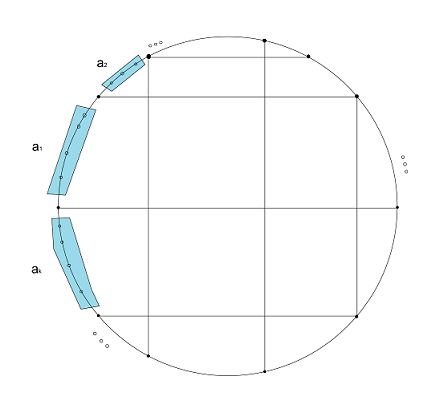
\includegraphics[scale=2.2]{problem_3}
\end{figure}
Dies lässt sich auch immer erreichen: Zeichne alle $n-3$ Diagonalen von einem Eckpunkt zu allen anderen Punkten ein. Eine dieser Diagonalen (eine Symmetrieachse des $n$-Ecks) verbindet den Ausgangspunkt mit dem Punkt, der diametral gegenüber liegt. Von diesem kann man die Nachbarspunkte wählen und verbinden, denn diese schneiden nur die Symmetrieachse und das in einem rechten Winkel. 

\textbf{Marking Scheme:}
\begin{itemize}
\item 1P: Keine rechtwinkligen Diagonalen bei $n$ ungerade
\item 2P: Nicht mehr als $n-3$ sich nicht schneidende Diagonalen in jedem konvexen $n$-Eck
\item 1P: Konstruktion für gerade und ungerade
\item 3P: Korrekte Argumentation für den Fall $n$ gerade
\end{itemize}
\end{itemize}

\newpage

\item[\textbf{4.}] %% Exercise 4 %%
Sei $k$ ein Kreis und $AB$ eine Sehne von $k$, sodass der Mittelpunkt von $k$ nicht auf $AB$ liegt. Sei $C$ ein von $A$ und $B$ verschiedener Punkt auf $k$. Für jede Wahl von $C$ seien $P_C$ und $Q_C$ die Projektionen von $A$ auf $BC$ respektive $B$ auf $AC$. Weiter sei $O_C$ der Umkreismittelpunkt des Dreiecks $P_{C}Q_{C}C$. Zeige, dass es einen Kreis $\omega$ gibt, sodass $O_C$ für jede Wahl von $C$ auf $\omega$ liegt.

\textbf{Lösung:}
Wir bemerken zuerst, dass $ABPQ$ wegen $\angle AQB = \angle APB = 90$ ein Sehnenviereck ist. Sei $M$ der Mittelpunkt der Sehne $AB$. Aus der Umkehrung von Thales im Dreieck $ABP$ folgt, dass $M$ der Umkreismittelpunkt von $ABPQ$ ist. \\
Wegen des Peripheriewinkelsatzes ist $\angle ACB$ unabhängig von der Wahl von $C$. Aufgrund des Zentriwinkelsatzes ist auch $\angle Q_CO_CP_C = 2\angle ACB$ unabhängig von $C$. Wegen der gleichschenkligen Dreiecke $AMQ$ und $MBP$ gilt:
\begin{align*}	
	\angle Q_CMP_C &= 180 - \angle BMP_C - \angle Q_CMA\\
	&=2(\angle ABC + \angle CAB) - 180\\
	&= 180 - \angle BCA.
\end{align*}
Also ist auch $\angle Q_CMP_C$ unabhängig von der Wahl von $C$. Da $Q_CM = P_CM$ nur von der Länge $AB$ abhängt, muss auch die Länge der letzten Seite $P_CQ_C$ des Dreiecks $P_CQ_CM$ von $C$ unabhängig sein. Weiter sieht man im Dreieck $Q_CO_CP_C$, dass $Q_CO_C = P_CO_C$ nicht von $C$ abhängen. Folglich hat das Viereck $Q_CO_CP_CM$ für jede Wahl von $C$ dieselbe Form. Insbesondere ist die Länge $O_CM$ konstant, also liegen alle $O_C$ auf einem Kreis mit Mittelpunkt $M$.

\textbf{Marking scheme:} \\
Die Punkte verschiedener Lösungen sind nicht additiv.
\begin{itemize}
\item Viereck $Q_CMP_CO_C$ hat immer die gleiche Form:
	\begin{itemize}
	\item $\angle Q_CMP_C$ unabhängig von $C$. +1P
	\item Länge $PQ$ unabhängig von $C$. +1P
	\item Länge $O_CP_C = O_CQ_C$ unabhängig von $C$. +2P
	\end{itemize}
\item $\omega$ ist Verschiebung von $k$ um $CO_C$
	\begin{itemize}
	\item $CO_C$ steht immer senkrecht auf $AB$. +1P
	\item Länge $PQ$ unabhängig von $C$. +1P
	\item Länge $CO_C$ unabhängig von $C$. +2P
	\end{itemize}
\item Mit $O_CH_C = \frac{CX}{2}$, $X = k \cap CO_C$
	\begin{itemize}
	\item $CO_C$ steht immer senkrecht auf $AB$. +1P
	\item $CO_C = O_CH$, wobei $H$ Höhenschnittpunkt. +1P
	\item $HH_C = H_CX$ und $C$, $H$, $X$ kollinear. +1P
	\end{itemize}
\end{itemize}
\newpage

\item[\textbf{5.}] %% Exercise 5 %%
Déterminer la plus petite constante réelle $C$ telle que pour tous $a_1,a_2,a_3,a_4,a_5\in \R_{>0}$, pas nécessairement distincts, il existe toujours quatre indices distincts $i,j,k,l$ tels que:
\[
\abs*{\frac{a_i}{a_j}-\frac{a_k}{a_l}}\leq C.
\]

\textbf{Solution:}
Après quelques essais, on remarque que $C=1/2$ est optimal.
\begin{itemize}
\item $C\geq 1/2$: en substituant $(1/2,1,1,1,n)$ et en laissant $n\rightarrow\infty$, on obtient $C\geq 1/2$.
\item $C\leq 1/2$: supposons que $a_5\geq a_4\geq\ldots\geq a_1$. On découpe $[0,1]$ en deux sous intervalles disjoints: $I=[0,1/2)$ et $J=[1/2,1]$. Regardons les fractions $0<\frac{a_1}{a_3},\frac{a_1}{a_5},\frac{a_3}{a_5}\leq 1$.\\
Si les trois fractions sont dans le même intervalle $I$ ou $J$, alors on remarque que cet intervalle contient aussi $\frac{a_2}{a_5}$ car $\frac{a_1}{a_5}\leq\frac{a_2}{a_5}\leq\frac{a_3}{a_5}$. Ainsi, $\frac{a_2}{a_5}$ et $\frac{a_1}{a_3}$ se trouve dans le même intervalle et donc à une distance inférieure à $1/2$.\\
Sinon, $I$ et $J$ contiennent au moins une des fractions $\frac{a_1}{a_3},\frac{a_1}{a_5},\frac{a_3}{a_5}$. Or $\frac{a_2}{a_4}$ se trouve soit dans $I$, soit dans $J$. On obtient à nouveau deux fractions avec indices différents dans le même intervalle. 
\end{itemize}

\textbf{Marking scheme:}
\begin{itemize}
\item $C\geq 1/2$ : 2P.
\item $C\leq 1/2$ : 5P, dont
\begin{itemize}
\item travailler avec $I$ et $J$ : 1P.
\item ordrer les valeurs et se concentrer sur les fractions $\leq 1$ : 1P.
\end{itemize}
\end{itemize}
\newpage


\item[\textbf{6.}] %% Exercise 6 %%
Trouver toutes les fonctions $f\colon\R_{>0}\to\R_{\geq0}$ telles que pour tous  $x,y\in\R_{>0}$:
\[
f(x)-f(x+y)=f(x^2f(y)+x).
\]

\textbf{Solution:}
Soit $f$ une solution de l'équation. On commence naturellement par chercher des fonctions qui sont solution. Après une petite recherche on trouve que les fonctions $x\mapsto 0$ et $x\mapsto 1/x$ marchent. De plus, comme $f(x^2f(y)+x)\geq 0$ la fonction est décroissante. Est-ce que la fonction peut-être strictement décroissante et donc injective ?
\begin{itemize}
\item $f$ est injective: pour bien utiliser l'injectivité, on trouve l'astuce suivante:
\[
f(x)-f(x+y)=f(x^2f(y)+x)=f(x)-f(x^2f(x^2f(y))+x),
\]
où l'on applique la formule $f(x+y)=f(x)-f(x^2f(y)+x)$ au terme $f(x+x^2f(y))$. Noter bien que cette manipulation est valable seulement si $f(y)\neq 0$ quelque soit $y$. Or en supposant que $f$ est injective, s'il existait $a>0$ avec $f(a)=0$, on aurait par décroissance $f(x)=0$ pour tout $x\geq a$ qui contredit l'injectivité.\newline
Ainsi après avoir simplifié par $f$, on obtient
\[
x+y=x^2f(x^2f(y))+x \,\Rightarrow\, y=x^2f(x^2f(y)).
\]
Substituer $y=1$ et $t=x^2f(1)$, donne $f(t)=f(1)/t$. En substituant dans l'équation de départ, on obtient $f(1)=1$ et donc la solution $t\mapsto 1/t$.
\item $f$ n'est pas injective: prenons $0<u<v$ avec $f(u)=f(v)$. Substituer $y=u$, puis $y=v$ donne $f(x+u)=f(x+v)$. Comme $f$ est décroissante, on obtient $f(x)=c$ pour tout $x>u$. Avec $x=y=v$, on obtient tout de suite $c=0$. Puis $x=y=u$ nous donne $f(u)=f(v)=0$. On a donc montré que pour $0<u<v$:
\[
f(u)=f(v)\Rightarrow f(u)=f(v)=0.
\]
On veut ici essayer de montrer que la fonction nulle est l'unique solution. On va donc chercher des "petites" valeurs de $x$ et $y$ telles que leur somme dépasse $u$. Par exemple, pour $x=y=u/2$, on obtient
\[
f\left(\frac{u}{2}\right)=f\left(\frac{u^2}{4}f\left(\frac{u}{2}\right)+\frac{u}{2}\right).
\]
Si $f(u/2)\neq 0$, alors on peut appliquer notre remarque ci-dessus pour en déduire que
\[
f\left(\frac{u}{2}\right)=f\left(\frac{u^2}{4}f\left(\frac{u}{2}\right)+\frac{u}{2}\right)=0.
\]
Contradiction. Donc on a bien $f(u/2)=0$. Par décroissance, $f(x)=0$ pour $x\geq u/2$. En poursuivant inductivement, on obtient $f(u/2^n)=0$ et donc que $f$ est la fonction nulle.
\end{itemize}
On obtient ainsi deux fonctions: $x\mapsto 0$ et $x\mapsto 1/x$. On vérifie qu'elles sont bien solutions.

\textbf{Marking scheme:}
\begin{itemize}
\item Cas $f$ injective : 2P, dont
\begin{itemize}
\item[-] $f(x+y)=f(x^2f(x^2f(y))+x)$ avec $f(y)\neq 0$ : 1P.
\end{itemize}
\item Cas $f$ non-injective :5P, dont
\begin{itemize}
\item[-] $0<u<v, f(u)=f(v)\Rightarrow f(u)=f(v)=0$ : 2P.
\end{itemize}
\item $f(a)=0\Rightarrow f(x)=0,\forall x\geq a$ ou $f$ décroissante : 0P.
\item solution complète sans vérification : 6P.
\end{itemize}
\newpage

\item[\textbf{7.}] %% Exercise 7 %%
Der brasilianische IMO-Leader wählt zwei natürliche Zahlen $n$ und $k$ mit $n>k$, und sagt diese dann seinem Deputy und einem Teilnehmer. Dann flüstert der Leader dem Deputy eine binäre Folge der Länge $n$ ins Ohr. Der Deputy schreibt alle binären Folgen der Länge $n$ auf, die sich genau an $k$ Stellen von der Folge des Leaders unterscheiden. (Beispiel für $n=3$ und $k=1$: Wenn der Leader $101$ wählt, schreibt der Deputy 001, 100, 111 auf.) Der Teilnehmer schaut sich die Folgen an, die der Deputy aufgeschrieben hat. Nun versucht der Teilnehmer, die ursprüngliche Folge vom Leader herauszufinden.
	
Wie viele Male muss er mindestens raten (abhängig von $n$ und $k$), bis er sicher einmal korrekt geraten hat?
	 
Bemerkung: Eine binäre Folge der Länge $n$ ist eine Folge der Länge $n$, die nur aus $0$ und $1$ besteht.

\textbf{Lösung:} Wenn wir eine fixe Stelle der Lösungsfolge $L$ betrachten, dann stimmen $\binom{n-1}{k}$ der aufgelisteten Folgen an dieser Stelle mit $L$ überein und $\binom{n-1}{k-1}$ der aufgelisteten Folgen unterscheiden sich an dieser Stelle von $L$. Da der Teilnehmer $n$ und $k$ kennt, kann er diese Werte auch ausrechnen. Zudem kann er zählen, wie viele der aufgeschriebenen Folgen eine $0$ bzw. $1$ an dieser Stelle aufweisen und daraus schliessen, ob in $L$ eine $0$ oder eine $1$ an der Stelle stand, sofern $\binom{n-1}{k} \neq \binom{n-1}{k-1}$ gilt. Dies kann er mit jeder Stelle tun, also ist die Lösungsfolge für ihn eindeutig und er benötigt nur einen Rateversuch. \\ \\ Falls $\binom{n-1}{k} = \binom{n-1}{k-1}$ gilt, dann gilt $n-k = k$, also $k = \frac{n}{2}$. In diesem Fall ist es leicht ersichtlich, dass die Lösungsfolge die gleiche Liste erzeugt wie ihr exaktes Gegenteil $L^{-1}$ (wenn man alle $0$ durch $1$ ersetzt und umgekehrt): Jede Folge, die auf der Liste von $L$ steht, unterscheidet sich an der Hälfte der Stellen von $L$, also unterscheidet sie sich an der anderen Hälfte der Stellen von $L^{-1}$ und steht somit auch auf der Liste von $L^{-1}$. Aus Symmetriegründen gilt das auch umgekehrt. Also sind die Listen von $L$ und $L^{-1}$ ununterscheidbar und die Anzahl Rateversuche ist mindestens $2$. Wir zeigen nun, dass es keine weitere Folge geben kann, die die gleiche Liste erzeugt. Dann kann der Teilnehmer durch Aufschreiben aller Möglichkeiten alle anderen Folgen ausschliessen und muss nicht öfter als $2$ Mal raten. \\
\\
Dafür rät der Teilnehmer die erste Zahl der Folge, OBdA eine $0$ (da sowohl $L$ als auch $L^{-1}$ Lösungen sind, führt dies sicher zu einer möglichen Lösung).
Dann streicht er alle $\binom{n-1}{k}$ Folgen, die mit einer $1$ beginnen und streicht bei allen anderen die $0$ an der ersten Stelle. Übrig bleiben (unter der Annahme, dass die $0$ richtig war) alle Folgen der Länge $n-1$, bei denen $k$ Einträge geändert wurden. Da $k \neq \frac{n-1}{2}$ gilt, ist die Lösung nun für den Teilnehmer nach dem ersten Fall eindeutig. Der Fall mit $1$ funktioniert komplett analog. Es kann also keine weiteren Lösungen geben.


\textbf{Marking scheme:}

\begin{list}{}{}
\item[•] $1$P: Es gibt $\binom{n-1}{k}$ Folgen auf der Liste, die an einer bestimmten Stelle mit $L$ übereinstimmen, bzw. $\binom{n-1}{k-1}$ Folgen, die sich an einer bestimmten Stelle von $L$ unterscheiden 
\item[•] $3$P insgesamt: Vollständige Argumentation im Fall $k \neq \frac{n}{2}$
\item[•] $1$P: Für $k=\frac{n}{2}$ erzeugt $L^{-1}$ die gleiche Liste wie $L$, also mindestens $2$ Versuche.
\item[•] $4$P insgesamt: Vollständige Argumentation im Fall $k=\frac{n}{2}$
\end{list}

\newpage

\item[\textbf{8.}] %% Exercise 8 %%
Finde alle monoton steigenden Folgen $a_1, a_2, a_3, \ldots$ natürlicher Zahlen, sodass $i+j$ und $a_i+a_j$ für alle $i,j \in \mathbb{N}$ die gleiche Anzahl Teiler haben.

\textbf{Lösung:} Erst zeigen wir, dass die Folge streng monoton steigend ist, dann, dass sie unendlich viele Fixpunkte enthält. Für eine natürliche Zahl $n$, sei $d(n)$ die Anzahl positiver Teiler von $n$.
\begin{itemize}
\item Streng monoton steigend: Nehme an, es gibt natürliche Zahlen $i<j$ sodass $a_i=a_j$; wegen Montonie führt dies zu $a_i=a_{i+1}$. Sei nun $k>2$ eine natürliche Zahl, sodass $i+k$ prim ist. Dann gilt
\[
2=d(i+k)=d(a_i+a_k)=d(a_{i+1}+a_k)=d(i+1+k).
\]
Da $i+k>2$ und prim ist, ist $i+1+k>2$ und gerade, somit nicht prim und daher $d(i+1+k)>2$, Widerspruch.
Alternative: Mit starker Induktion und Bertrand kann man $a_i\equiv i \mod 2$ für alle natürlichen $i$ zeigen, was auch zu strenger Montonie führt.
\item Unendlich viele Fixpunkte: Sei $p$ eine Primzahl, dann gilt
\[
p=d(2^{p-1})=d(2^{p-2}+2^{p-2})=d(a_{2^{p-2}}+a_{2^{p-2}})=d(2a_{2^{p-2}}).
\]
Betrachtet man dann die Primfaktorzerlegung $2a_{2^{p-2}}=\prod_{i=1}^r p_i^{\alpha_i}$ mit $\alpha_1,...,\alpha_i>0$, so haben wir also $p=\prod_{i=1}^r(1+\alpha_i)$, was wegen $p$ prim zu $r=1$ und $\alpha_1=p-1$ führt. Da aber natürlich $2$ ein Teiler ist von $2a_{2^{p-2}}$, gilt zusätzlich $p_1=2$ und somit $2a_{2^{p-2}}=2^{p-1}\implies a_{2^{p-2}}=2^{p-2}$.
\item Konklusion: Wegen strenger Monotonie gilt $a_{i+d}\geq d+a_{i}$, insbesondere $a_i\geq i$, für alle $i,d\in\mathbb{N}$.  Nehme an, es gibt ein $i\in\mathbb{N}$ sodass $a_i>i$. Man wählt dann $p$ prim so, dass $2^{p-2}>i$, dann erhält man
\[
2^{p-2}=a_{2^{p-2}}\geq 2^{p-2}-i+a_i>2^{p-2},
\]
Widerspruch. Somit gilt $a_i=i$ für alle natürlichen $i$ und man sieht leicht, dass diese Folge die Bedingungen erfüllt.

\textbf{Marking Scheme:}
\begin{itemize}
\item streng monoton steigend: 2 Punkte, davon
\begin{itemize}
\item 1 Punkt, wenn man aus $a_i=a_j$ mit $i\neq j$ Periodizität von $d$ zeigt, oder
\item 1 Punkt für $a_i\equiv i \mod 2$ für alle $i$
\end{itemize}
\item unendlich viele Fixpunkte: 3 Punkte
\item fertig machen: 2 Punkte
\item Keine Punkte: $a_i$ für kleine $i$ berechnen und Aussagen, die direkt aus diesen Berechnungen folgen, $a_p$ prim für $p$ prim.
\end{itemize}
\newpage

\item[\textbf{9.}] %% Exercise 9 %%
Soit $ABC$ un triangle avec $AB=AC\neq BC$ et $I$ le centre de son cercle inscrit. La droite $BI$ coupe $AC$ en $D$, et la perpendiculaire à $AC$ passant par $D$ coupe $AI$ en $E$. Montrer que la réflexion de $I$ par rapport à la droite $AC$ est sur le cercle circonscrit au triangle $BDE$.

\textbf{Solution 1:}
On note $I'$ le symétrique de $I$ par rapport à $AC$, $J$ et $F$ les symétriques respectifs de $I$ et $C$ par $D$, $M$ le milieu de $II'$, $A'$ le milieu de $BC$, $S$ l'intersection de $AI$ et $I'C$, $K$ l'intersection de $II'$ avec la médiatrice de $BI$ et $\Gamma$ le cercle de centre $E$ passant par $B$ (et $E$).

Comme $ED$ est perpendiculaire à $AC$, on a que $F\in \Gamma$. $\angle DCI=\angle ICB=\angle CBI$ nous donne que $DC$ est tangent au cercle circonscrit de $IBC$. On a donc
\[DF\cdot DC= DC^2= DI\cdot DB =DJ\cdot DB\]
et ainsi $J \in \Gamma$. Comme $IJ$ et $CF$ se coupent en leur milieu, $CJFI$ est un parralèlogramme. Par conséquent $\angle FI'C=\angle CIF =\angle FJC$, et ainsi $I' \in \Gamma$. Alors $EI'=EB$. Ainsi $E$ est sur la bissectrice extérieure de l'angle en $D$ du triangle $BDI'$ et sur la médiatrice du coté $BI'$. Il est donc sur le cercle circonscrit de $BDI'$.

\textbf{Solution 2:}

Soit $\theta = \angle ACI = \angle ICB =\angle CBI$. On a alors
\[
\angle I'SE=\angle I'CA + \angle CAI= \theta + \( \frac{\pi}{2} +2\theta \) = 3 \theta + 90^\circ
\]
et
\[
\angle I'DE = \angle I'DC + 90^\circ =\angle CDI + 90^\circ = \angle DCB + \angle CBD + 90^\circ =3 \theta + 90^\circ
\]
Donc $I'DES$ est inscrit. Par ailleurs, on a $\angle I'SB= 2 \angle I'SE=6\theta$ et $\angle I'DB= 2\angle CDI= 6 \theta$. Donc $I'DBS$ est inscrit, tout comme $I'DES$, ce qui démontre l'énoncé.

%\textbf{Solution 3:}

\textbf{Marking Scheme:}
\begin{itemize}
\item première solution
\begin{itemize}
\item $F \in \Gamma$: \hfill 1P.
\item $J\in \Gamma$: \hfill +1P.
\item $I'\in \Gamma$: \hfill +2P.
\item Réduire le problème à: $BEI'$ est isocèle: \hfill 1P.
\end{itemize}
\item deuxième solution
\begin{itemize}
\item Trouver un quadrilatère inscrit parmi $B$, $D$, $E$ $I'$ et $S$: \hfill 3P.
\item Trouver un autre quadrilatère inscrit parmi les mêmes points: \hfill 3P.
\item Conclure: \hfill 1P.
\end{itemize}
%\item troisième solution
%\begin{itemize}
%\item $BKDI'$ est un quadrilatère inscrit : \hfill 2P.
%\item $KI=DE$ : \hfill 2P.
%\item $KIDE$ est un parallélogramme: \hfill +1P.
%\item $BKED$ est un quadrilatère inscrit: \hfill +1P.
%
%\end{itemize}

\end{itemize}
\newpage

\item[\textbf{10.}] %% Exercise 10 %%
Trouver tous les polynômes $P$ à coefficients entiers tels que $P(2017n)$ est un nombre premier pour tout nombre naturel $n$.

\textbf{Solution:} Puisque $P$ est un polynôme à coefficients entiers, on a que $a-b\div P(a) - P(b)$ pour tous $a, b\in \Z$. Ainsi en particulier nous avons que, pour $q=P(2017)$,  $P(2017kq + 2017) \equiv P(2017) \mod {q}$, mais par hypothèse ces deux valeurs sont des nombres premiers, donc on a $P(2017kq + 2017) = P(2017)$ pour une infinité de $k$, donc $P$ est constant.

\textbf{Marking Scheme:}
\begin{itemize}
\item Si $\deg(P) \geq 1$, alors $P(0) = \pm 1$: \hfill 1P.
\item Substituer $Q(n) = P(n+2017)$ et remarquer que $Q(0)$ est un nombre premier: \hfill +2P.

\item $P(2017kq + 2017) \equiv P(2017) \mod q$:\hfill 3P.
\end{itemize}

\newpage

\item[\textbf{11.}] %% Exercise 11 %%

Seien $B=(-1,0)$ und $C=(1,0)$ fixe Punkte in der Ebene. Eine nichtleere, beschränkte Teilmenge $S$ der Ebene heisst \emph{nett}, falls die folgenden Bedingungen gelten:

\begin{enumerate}[(i)]
\item Es gibt einen Punkt $T$ in $S$, sodass für jeden anderen Punkt $Q$ in $S$ die Strecke $TQ$ vollständig in $S$ liegt.
\item Für jedes Dreieck $P_1P_2P_3$ existiert ein eindeutiger Punkt $A$ in $S$ und eine Permutation $\sigma$ von $\{1, 2, 3\}$, sodass die Dreiecke $ABC$ und $P_{\sigma(1)}P_{\sigma(2)}P_{\sigma(3)}$ ähnlich sind.
\end{enumerate}

Zeige, dass es zwei verschiedene nette Teilmengen $S$ und $S'$ der Menge $\{(x,y):x\geq 0,y\geq 0\}$ mit folgender Eigenschaft gibt: Das Produkt $BA\cdot BA'$ ist unabhängig von der Wahl des Dreiecks $P_1P_2P_3$, wobei $A\in S$ und $A'\in S'$ jeweils die eindeutigen Punkte aus (ii) für ein beliebiges Dreieck $P_1P_2P_3$ sind.

\textbf{Lösung (Cyril):}Seien $k_B$ und $k_C$ zwei Kreise um $B$ bzw. $C$ mit Radius 2. Wir definieren die zwei Gebiete $S$ und $S'$ folgendermassen:
\[
S = \{ p=(x,y) : x \geq 0, y \geq 0, \text{dist}(B,p) \leq 2 \}
\]
\[
S' = \{ p=(x,y) : x \geq 0, y \geq 0, \text{dist}(C,p) \leq 2,  \text{dist}(B,p) \geq 2 \}
\]

\begin{center}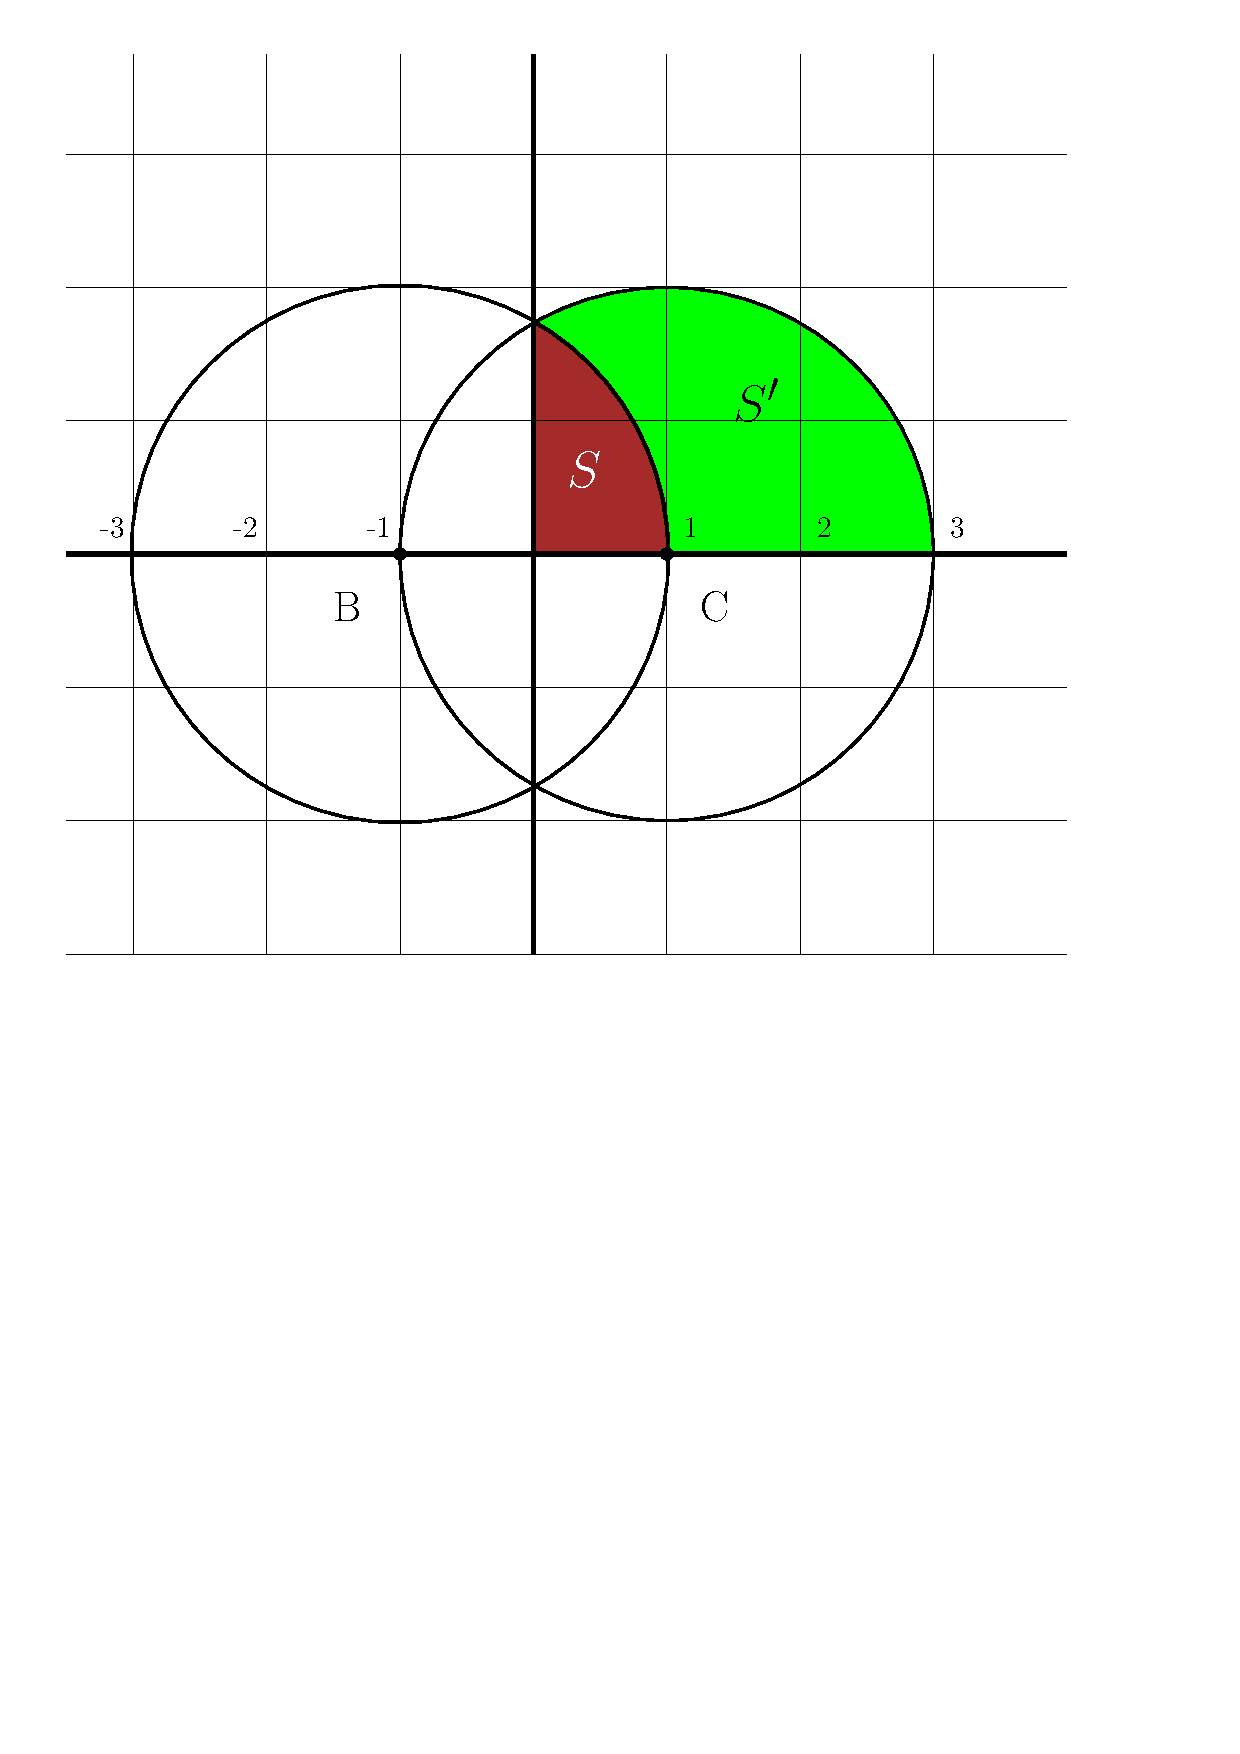
\includegraphics[scale=0.7]{2017_11}\end{center}

Die Gebiete sind in der Skizze eingezeichnet. Offensichtlich erfüllen beide Gebiete die Bedingung $(i)$. Um Bedingung $(ii)$ zu zeigen nehmen wir nun an, wir haben ein Dreieck $P_1P_2P_3$ gegeben mit den Streckenlängen $a\leq b \leq c$.

Wir suchen nun ein Dreieck $ABC$ mit Streckenlängen $a' \leq b' \leq c'$ das ähnlich zu $P_1P_2P_3$ ist. Unsere erste Beobachtung ist, dass $AC$ nicht strikt grösser sein darf als $AB$, da sonst $A$ nicht im ersten Quadranten ($x\geq 0, y \geq 0$) liegt. Das heisst wir dürfen die längste Seite $c'$ nicht als $AB$ wählen.

Wir haben daher zwei Möglichkeiten:

\begin{enumerate}[1.]
\item $BC = c'$
\item $AB = c'$
\end{enumerate}

Im ersten Fall folgt noch $AB = b'$, $AC = a'$ (wieder da $AC$ kleiner als $AB$ sein muss). Im zweiten wählen wir noch $BC = b'$, $AC = a'$ (hier hätten wir auch eine andere Möglichkeit, aber unsere funktioniert um $BA\cdot BA' = 4$ zu zeigen).

Dies definiert uns für jedes Dreieck einen eindeutigen Punkt $A$.

Wir können nun sehen, dass wir im ersten Fall $A \in S'$ haben. Denn da $AC \leq BC$ muss $A$ im Kreis $k_C$ liegen (mit dem Extremfall eines gleichschenkligen Dreieck mit $b' = c'$, bei dem $A$ auf dem Kreis liegt). Aussderem darf $A$ nicht im Kreis $k_B$ liegen, da wir $BC \leq AB$ haben (mit dem Extremfall eines gleichschenkligen Dreeicks mit $a' = b'$, bei dem $A$ auf dem Kreis $k_B$ liegt). 

Ausserdem haben wir für jeden Punkt in $S'$ die Bedingung an die Strecken erfüllt, das heisst das Gebiet $S'$ erfüllt die Bedingung $(ii)$.

Fast gleich können wir zeigen, dass das Gebiet $S$ die Bedingung $(ii)$ erfüllt, wenn wir die zweite Möglichkeit wählen.

\textit{Bemerkung: Im Fall eines gleichseitigen Dreiecks oder einen gleichschenkligen Dreiecks mit $a' = b'$ sind die beiden Möglichkeiten identisch und wir erhalten $A = S \cap S'$.}

Wenn wir das Beispiel des gleichseitigen Dreiecks nehmen, bemerken wir auch dass $BA \cdot BA' = 4$ gelten muss. Wir können nun die Ähnlichkeit ($\frac{a'}{a}=\frac{b'}{b}=\frac{c'}{c}$) und $BC = 2$ benutzen um dies für beliebige Dreiecke zu zeigen:

Im ersten Fall haben wir $BC = c'$ und $AB = b'$, also
\[
\frac{AB}{BC} = \frac{b'}{c'} = \frac{b}{c} \iff AB = \frac{b}{c}\cdot 2.
\]

Im zweiten Fall haben wir $BC = b' = 2$ und $AB = c'$, also
\[
\frac{A'B}{BC} =\frac{c'}{b'} = \frac{c}{b} \iff A'B = \frac{c}{b}\cdot 2
\]

Zusammen also $AB \cdot A'B = 4$. \qed

\textbf{Marking Scheme:}

\begin{itemize}
\item Nicht additiv:
\begin{itemize}
\item 1 Punkt: $BA \cdot BA' = 4$ beweisen 
\item 1 Punkt: $S \cap S'$ bestimmen.
\item 3 Punkte: $S$ und $S'$ definieren.
\end{itemize}
\end{itemize}
\item 1 Punkt: $S$ oder $S'$ definieren und $(i), (ii)$ beweisen.
\item 1 Punkt: $S$ und $S'$ definieren und $(i), (ii)$ beweisen.
\item 2 Punkte: $S$ und $S'$ definieren und $BA \cdot BA' = const.$ beweisen unter Annahme von $(i), (ii)$ 
\end{itemize}
\newpage

\item[\textbf{12.}] %% Exercise 12 %%
Soient $a, c\in  \N$ et $b\in \Z$. Prouver qu'il existe $x\in \N$ tel que
\[
a^x+x\equiv b \mod c.
\]

\textbf{Solution:} Supposons dans un premier temps que $c = p^n$ est une puissance d'un nombre premier. Nous allons construire une suite $(x_1, \ldots, x_n)$ telle que pour tout $1\leq k\leq n$ on ait $a^{x_k} + x_k \equiv b \mod {p^k}$ et $x_k \equiv x_{k-1} \mod {(p-1)p^{k-1}}$. Rappelons que $\phi(p^n) = (p-1)p^{n-1}$.
		
Si $p|a$, alors $p|a^x$ et donc on peut prendre $x_1\equiv b\mod p$. Écrivons $x_{k+1} = x_k + \lambda (p-1)p^k$. Alors
\[
	a^{x_{k+1}}+x_{k+1} = a^{\lambda (p-1)p^k}a^{x_k} + \lambda (p-1)p^k + x_k \equiv -\lambda p^k + x_k \mod{p^{k+1}}
\]
car clairement $a^{\lambda (p-1)p^k} \equiv 0 \mod{p^{k+1}}$ et ainsi il suffit de choisir $0\leq \lambda < p$ de telle sorte que $\lambda \equiv (x_k-b)/p^k \mod{p}$. Ainsi cela nous donne la suite voulue. De plus, tous les nombres $x_k$ sont congruents à $x_1$ modulo $p-1$ par construction et comme $p$ et $p-1$ sont premiers entre eux $x_1$ peut prendre n'importe quel reste modulo $p-1$.

Si $p\ndiv a$, commençons par $x_0$ n'importe quel nombre parmi $1, 2, \ldots, p-1$. Ensuite pour $1\leq k \leq n$ supposons qu'on ait déjà trouvé $x_{k-1}$ et cherchons un $x_k$ de la forme $x_k = \lambda (p-1)p^{k-1} + x_{k-1}$. On a alors
\[
	a^{x_k} + x_k = a^{\lambda(p-1)p^{k-1}}a^{x_{k-1}} + \lambda(p-1)p^{k-1}+ x_{k-1}\equiv 
	a^{x_{k-1}} - \lambda p^{k-1} + x_{k-1} \mod{p^{k}}
\]
et, puisque $x_{k-1}$ est une solution modulo $p^{k-1}$ on peut choisir $\lambda = \frac{a^{x_{k-1}}+x_{k-1}-b}{p^{k-1}}$. On obtient alors la suite voulue et par construction $x_n \equiv x_0 \mod{p-1}$ donc $x_n$ peut prendre n'importe quel reste modulo $p-1$.

Dans le cas général, nous pouvons écrire $c = p_1^{\alpha_1}\cdot\ldots \cdot p_k^{\alpha_k}$ avec les $p_i$ en ordre croissant. Nous procédons par induction sur le nombre $k$ de facteurs premiers pour montrer qu'il y a une solution $x$ modulo $d_k = \kgV(c, \phi(c))$.
\begin{itemize}
	\item Si $k = 0$, i.e. $c = 1$, le résultat est trivialement vrai quel que soit $x$.
	\item Si $k = 1$, i.e. $c = p^n$ pour un certain nombre premier $p$ et $n \geq 1$, nous avons déjà prouvé l'existence d'un tel $x$ dans la partie précédente et on voit facilement que si $x$ augmente ou diminue de $(p-1)p^{n} = p\phi(p^n)$ on a toujours une solution.
	\item Supposons maintenant qu'on a déjà trouvé une solution $x$ pour $c_{n-1} = p_1^{\alpha_1}\cdot\ldots\cdot p_{n-1}^{\alpha_{n-1}}$ et soit $d_{n-1}$ défini comme précédemment. Considérons $d = \ggT(d_{n-1}, p_n\phi(p_n^{\alpha_n}))$. Nous pouvons alors choisir une solution $y$ à l'équation modulo $p_n^{\alpha_n}$ et nous pouvons de plus supposer que $y\equiv x \mod{d}$ (car $y$ peut prendre n'importe quelle valeur modulo $p_n - 1$ et $p_n$ est premier avec $d_{n-1}$). Nous pouvons écrire $d_{n-1} = f'g$ et $(p_n - 1)p_n^{\alpha_n} = f'' h$ de telle manière que $g, h$ soient premier avec $d$ et les facteurs premiers de $f',f''$ soient précisément ceux de $d$. En particulier $g$ et $h$ sont premiers entre eux et on définit $f = \kgV(f', f'')$. Le théorème des restes chinois nous assure l'existence d'une solution $z$ modulo $fgh$ au système de congruences
	\[
		z\equiv x \mod{f},\qquad z\equiv x \mod g,\qquad z\equiv y \mod h.
	\]
	
	Alors, par construction, on a que $z\equiv x \mod{d_{n-1}}$ et $z\equiv y \mod{(p_n - 1)p_n^{\alpha_n}}$ donc $z$ est notre solution recherchée à l'équation modulo $p_1^{\alpha_1}\cdot\ldots\cdot p_n^{\alpha_n}$. De plus on voit par construction que $fgh = \kgV(d_{n-1}, (p_n - 1)p_n^{\alpha_n}) = d_n$.
\end{itemize}

\textbf{Marking Scheme:}
\begin{itemize}
\item Trouver une solution dans le cas $c=p$: \hfill 1P.
\item Trouver une solution dans le cas $c=p^k$: \hfill +2P.
\item Conclure : \hfill 7P.
\end{itemize}


\end{enumerate}
\end{document}
